\textbf{1-1.} 氢原子由一个质子（即氢原子核）和一个电子组成。根据经典模型，在正常状态下，电子绕核作圆周运动，轨道半径是 $5.29 \times 10^{-11} \mathrm{~m}$ 。已知质子质量 $m_{\mathrm{p}} = 1.67 \times 10^{-27} \mathrm{~kg}$ ，电子质量 $m_{\mathrm{e}} = 9.11 \times 10^{-31} \mathrm{~kg}$ ，电荷分别为 $\pm e = \pm 1.60 \times 10^{-19} \mathrm{C}$ ，万有引力常量 $G = 6.67 \times 10^{-11} \mathrm{~N} \cdot \mathrm{m}^{2} / \mathrm{kg}^{2}$ 。

(1) 求电子所受质子的库仑力和引力；

(2) 库仑力是万有引力的多少倍？

(3) 求电子的速度。

\vfill

\textbf{1-2.} 卢瑟福实验证明: 当两个原子核之间的距离小到 $10^{-15}$ m 时, 它们之间的排斥力仍遵守库仑定律。金的原子核中有 79 个质子, 氦的原子核 (即 $\alpha$ 粒子) 中有 2 个质子。已知每个质子带电荷量 $e = 1.60 \times 10^{-19}$ C, $\alpha$ 粒子的质量为 $6.68 \times 10^{-27}$ kg。当 $\alpha$ 粒子与金核相距为 $6.9 \times 10^{-15}$ m 时 (设这时它们都仍可当作点电荷), 求 

(1) $\alpha$ 粒于所受的力; 

(2) $\alpha$ 粒子的加速度。

\vfill
\newpage

\textbf{1-3.} 铁原子核里两质子相距 $4.0 \times 10^{-15} \mathrm{~m}$ , 每个质子带电荷量 $e = 1.60 \times 10^{-19} \mathrm{C}$ ,

(1) 求它们之间的库仑力; 

(2) 比较这力与每个质子所受重力的大小。

\vfill

\textbf{1-4.} 两小球质量都是 $m$ ，都用长为 $l$ 的细线挂在同一点；若它们带上相同的电量，平衡时两线夹角为 $2\theta$ （见本题图）。设小球的半径都可略去不计，求每个小球上的电量。
\begin{center}
    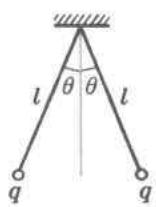
\includegraphics[width=0.15\linewidth]{figures/习题1-4.jpg}
\end{center}

\vfill
\newpage

\textbf{1-5.} 电子所带的电荷量(基元电荷 $-e$ ) 最先是由密立根通过油滴实
验测出的。密立根设计的实验装置如本题图所示。一个很小的带电油滴在电场 E 内。调节 E，使作用在油滴上的电场力与油滴所受的重力平衡，如果油滴的半径为 $1.64 \times 10^{-4}$ cm，在平衡时， $E=1.92\times10^{5}N/C$ . 求油滴上的电荷(已知油的密度为0.851g/cm $^{3}$ )
\begin{center}
    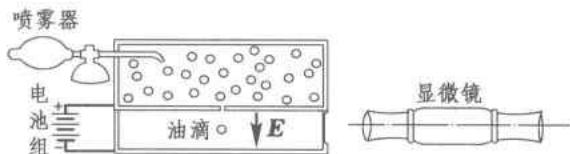
\includegraphics[width=\linewidth]{figures/习题1-5.jpg}
\end{center}
\vfill

\textbf{1-6.} 在早期(1911年)的一连串实验中,密立根在不同时刻观察单个油滴上呈现的电荷,其测量结果(绝对值)如下:
$$
\begin{array}{l l l} 6. 5 6 8 \times 1 0 ^ {- 1 9} \mathrm{C} & 1 3. 1 3 \times 1 0 ^ {- 1 9} \mathrm{C} & 1 9. 7 1 \times 1 0 ^ {- 1 9} \mathrm{C} \\ 8. 2 0 4 \times 1 0 ^ {- 1 9} \mathrm{C} & 1 6. 4 8 \times 1 0 ^ {- 1 9} \mathrm{C} & 2 2. 8 9 \times 1 0 ^ {- 1 9} \mathrm{C} \\ 1 1. 5 0 \times 1 0 ^ {- 1 9} \mathrm{C} & 1 8. 0 8 \times 1 0 ^ {- 1 9} \mathrm{C} & 2 6. 1 3 \times 1 0 ^ {- 1 9} \mathrm{C} \end{array}
$$
根据这些数据,可以推得基元电荷 e 的数值为多少?

\vfill
\newpage

\textbf{1-7.} 根据经典理论，在正常状态下，氢原子中电子绕核作圆周运动，其轨道半径为 $5.29 \times 10^{-11} \mathrm{~m}$ 。已知质子电荷为 $e = 1.60 \times 10^{-19} \mathrm{C}$ ，求电子所在处原子核（即质子）的电场强度。


\vfill

\textbf{1-8.} 如本题图，一电偶极子的电偶极矩 $p = ql$ ， $P$ 点至偶极子中心 $O$ 的距离为 $r$ ， $r$ 与 $l$ 的夹角为 $\theta$ . 设 $r \gg l$ ，求 $P$ 点的电场强度 $E$ 在 $r = \overrightarrow{OP}$ 方向的分量 $E_r$ 和垂直于 $r$ 方向上的分量 $E_\theta$ .
\begin{center}
    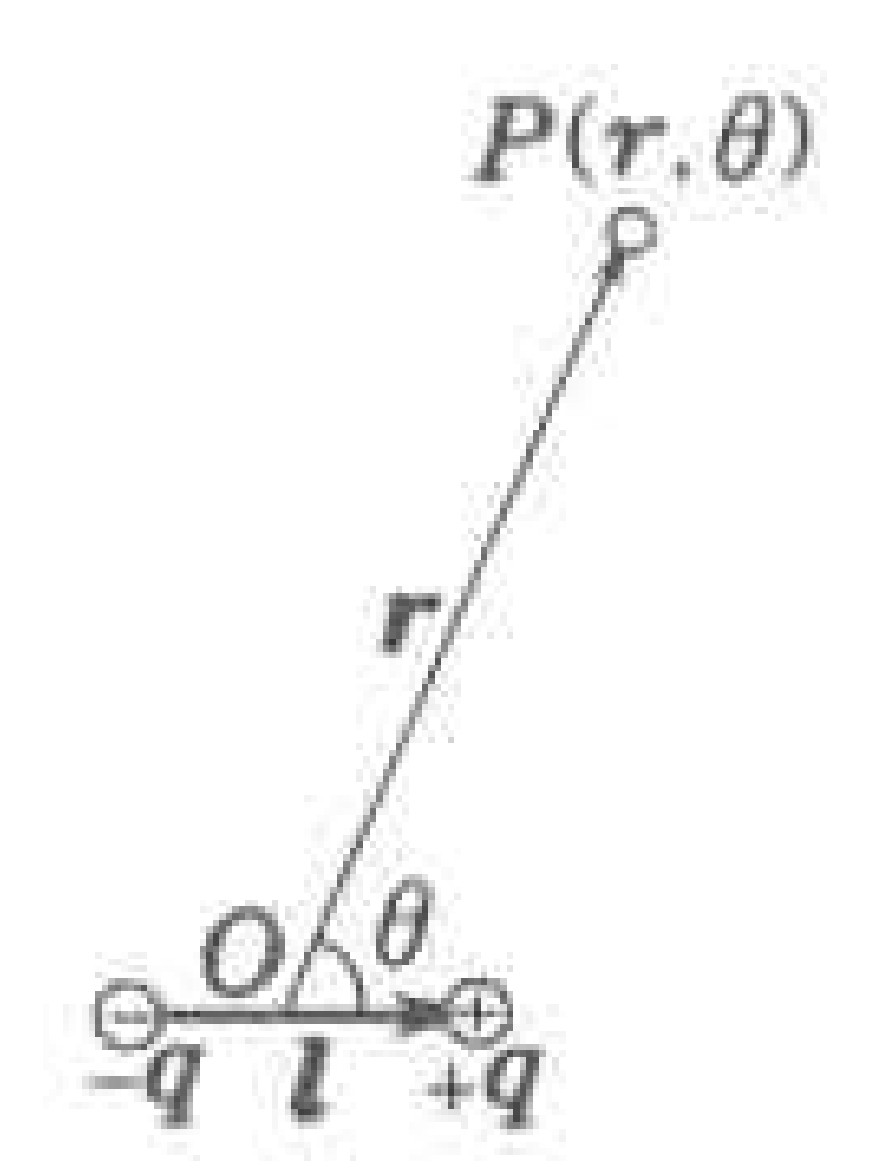
\includegraphics[width=0.2\linewidth]{figures/习题1-8.jpg}
\end{center}

\vfill
\newpage

\textbf{1-9.} 把电偶极矩为 $p = ql$ 的电偶极子放在点电荷 $Q$ 的电场内， $p$ 的中心 $O$ 到 $Q$ 的距离为 $r(r \gg l)$ 。分别求 (1) $p // \overrightarrow{QO}$ (本题图 a) 和 (2) $p \perp \overrightarrow{QO}$ (图 b) 时偶极子所受的力 $F$ 和力矩 $L$ .
\begin{center}
    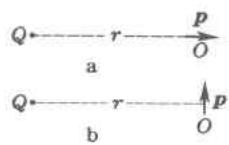
\includegraphics[width=0.3\linewidth]{figures/习题1-9.jpg}
\end{center}

\vfill

\textbf{1-10.} 本题图中所示是一种电四极子，它由两个相同的电偶极子 $p = q \, l$ 组成，这两个偶极子在一直线上，但方向相反，它们的负电荷重合在一起。试证明：在它们的延长线上离中
心（即负电荷）为 $r(r \gg l)$ 处，

(1) 场强为 $E = \frac{3Q}{4\pi\varepsilon_{0}r^{4}}$ ,

(2) 电势为 $U(r)=\frac{Q}{4\pi\varepsilon_{0}r^{3}}$ ,
式中 $Q=2ql^{2}$ 叫做它的电四极矩。
\begin{center}
    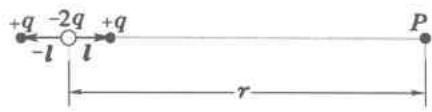
\includegraphics[width=0.5\linewidth]{figures/习题1-10a.jpg}
\end{center}

\vfill
\newpage

\textbf{1-11.} 本题图中所示是另一种电四极子，设 $q$ 和 $l$ 都已知，图中 $P$ 点到电四极子中心 $O$ 的距离为 $x(x \gg l)$ , $\overrightarrow{OP}$ 与正方形的一对边平行, 求 $P$ 点的电场强度 $E$.

\begin{center}
    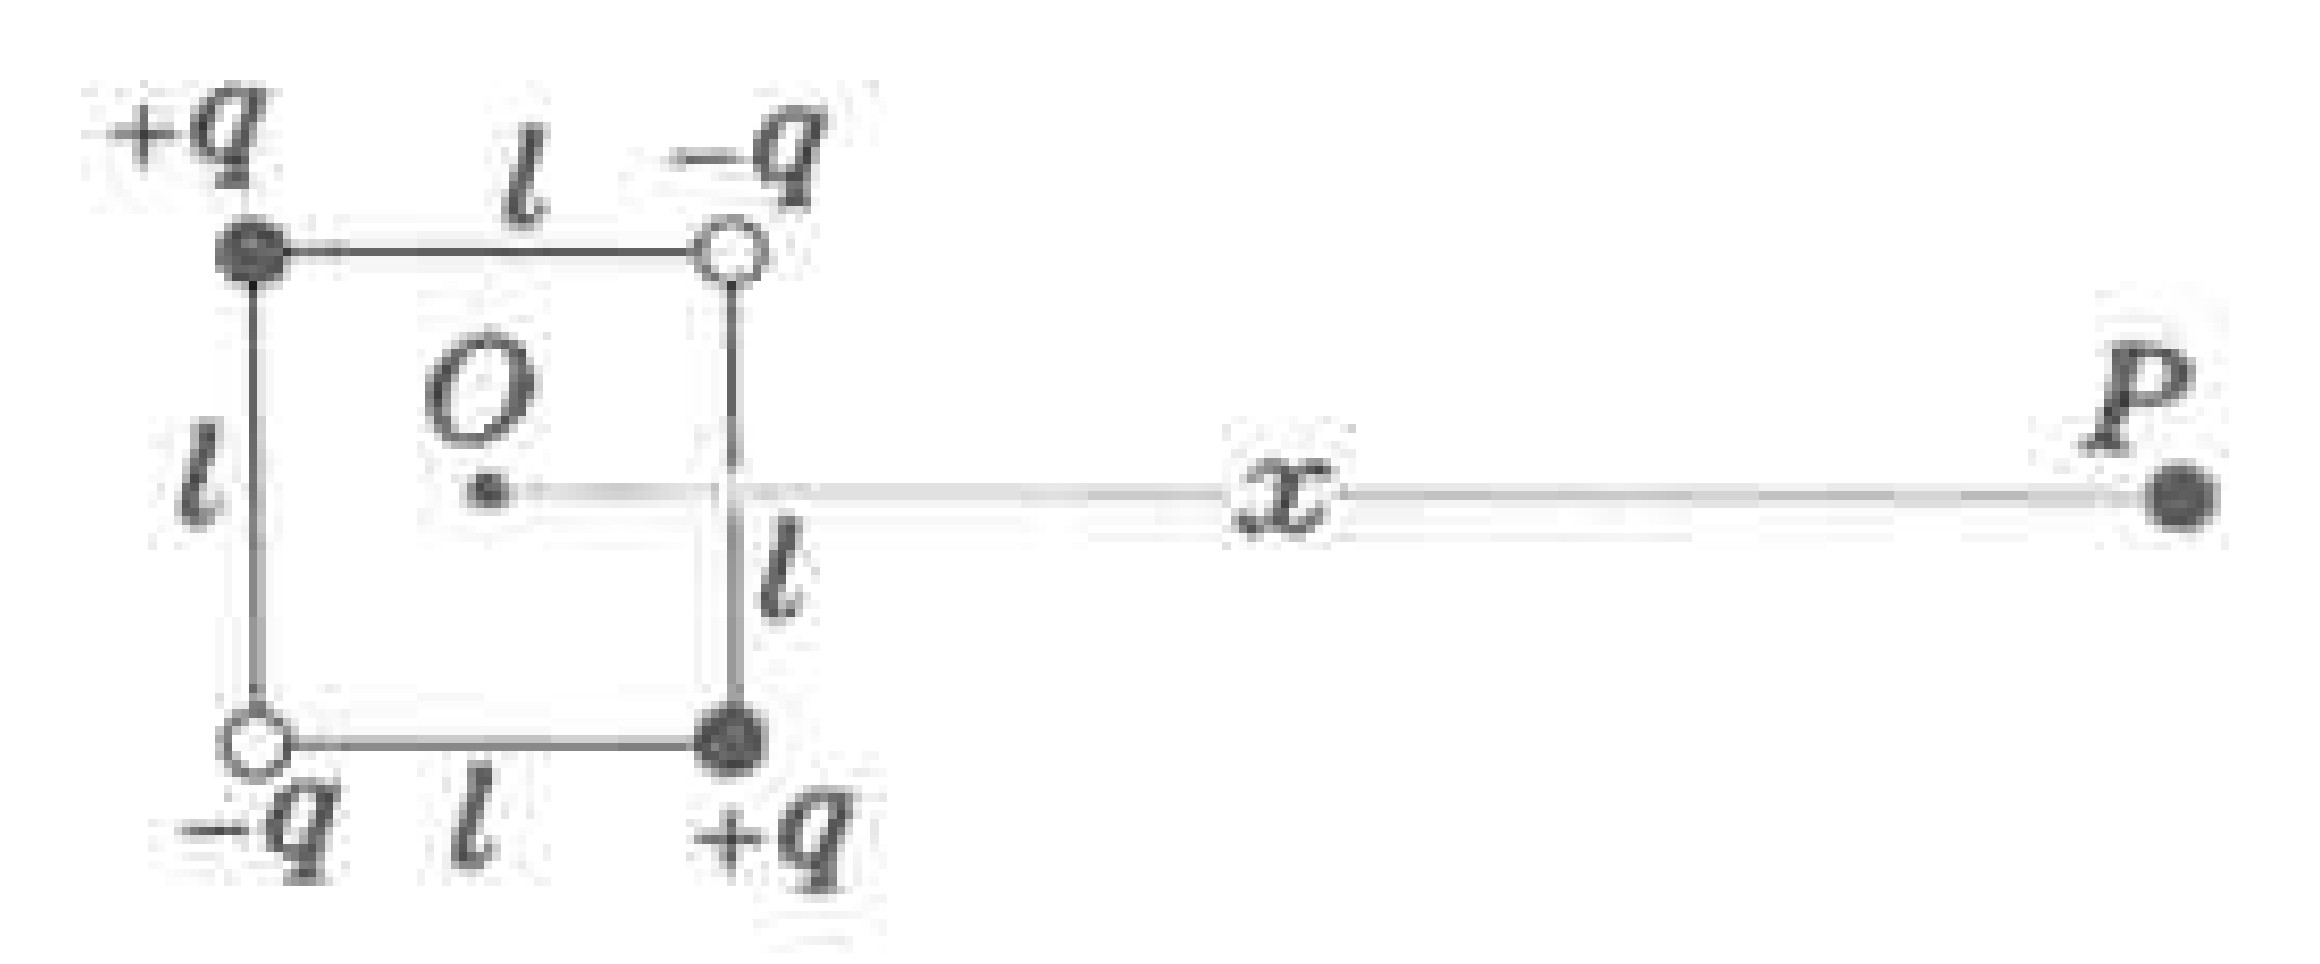
\includegraphics[width=0.3\linewidth]{figures/习题1-11.jpg}
\end{center}

\vfill

\textbf{1-12.} 两条平行的无限长直均匀带电线，相距为 $a$ ，电荷线密度分别为 $\pm \eta_{\mathrm{e}}$ 

（1）求这两线构成的平面上任一点（设这点到其中一线的垂直距离为 $x$ ）的场强；

（2）求每线单位长度上所受的相互吸引力。

\vfill
\newpage

\textbf{1-14.} 根据量子理论, 氢原子中心是个带正电 $e$ 的原子核(可看成点电荷), 外面是带负电的电子云。在正常状态(核外电子处在 s 态)下, 电子云的电荷密度分布球对称:
$$
\rho_ {\mathrm{e}} = - \frac {e}{\pi a _ {\mathrm{B}} ^ {3}} \mathrm{e} ^ {- 2 r / a _ {\mathrm{B}}},
$$
式中 $a_{B}$ 为一常量（它相当于经典原子模型中电子圆形轨道的半径，称为玻尔半径）。求原子内的电场分布。

\vfill

\textbf{1-15.} 实验表明: 在靠近地面处有相当强的电场, $E$ 垂直于地面向下, 大小约为 $100 \mathrm{~V} / \mathrm{m}$ ; 在离地面 $1.5 \mathrm{~km}$ 高的地方, $E$ 也是垂直于地面向下的, 大小约为 $25 \mathrm{~V} / \mathrm{m}$ .

(1) 试计算从地面到此高度大气中电荷的平均体密度；

(2) 如果地球上的电荷全部均匀分布在表面, 求地面上电荷面密度。

\vfill
\newpage

\textbf{1-16.} 半径为 $R$ 的无穷长直圆筒面上均匀带电，沿轴线单位长度的电量为 $\lambda$ 。求场强分布，并画出 $E - r$ 曲线。

\vfill

\textbf{1-17.} 两无限大的平行平面均匀带电，电荷的面密度分别为 $\pm \sigma_{\mathrm{e}}$ ，求各区域的场强分布。

\vfill
\newpage

\textbf{1-18.} 两无限大的平行平面均匀带电，电荷面密度都是 $\sigma_{\mathrm{e}}$ ，求各处的场强分布。

\vfill

\textbf{1-19.} 三个无限大的平行平面都均匀带电，电荷面密度分别为 $\sigma_{\mathrm{el}}$ 、 $\sigma_{\mathrm{e2}}$ 、 $\sigma_{\mathrm{e3}}$ 。求下列情况各处的场强：

(1)$\sigma_ {\mathrm{e} 1} = \sigma_ {\mathrm{e} 2} = \sigma_ {\mathrm{e} 3} = \sigma_ {\mathrm{e}};$

(2) $\sigma_{\mathrm{e1}} = \sigma_{\mathrm{e3}} = \sigma_{\mathrm{e}}; \sigma_{\mathrm{e2}} = -\sigma_{\mathrm{e}};$

(3) $\sigma_{\mathrm{e1}} = \sigma_{\mathrm{e3}} = -\sigma_{\mathrm{e}}; \sigma_{\mathrm{e2}} = \sigma_{\mathrm{e}};$

(4) $\sigma_{\mathrm{e1}} = \sigma_{\mathrm{e}}, \sigma_{\mathrm{e2}} = \sigma_{\mathrm{e3}} = -\sigma_{\mathrm{e}}.$

\vfill
\newpage

\textbf{1-20.} 一厚度为 $d$ 的无限大平板，平板体内均匀带电，电荷体密度为 $\rho_0$ 。求板内、外场强的分布。

\vfill

\textbf{1-21.} 在夏季雷雨中,通常一次闪电里两点间的电势差约为 $100\mathrm{MV}$ , 通过的电量约为 $30\mathrm{C}$ . 问一次闪电消耗的能量是多少? 如果用这些能量来烧水,能把多少水从 $0^{\circ}\mathrm{C}$ 加热到 $100^{\circ}\mathrm{C}$ ?

\vfill
\newpage

\textbf{1-23.} 求一对等量同号点电荷联线中点的场强和电势, 设电荷都是 $q$, 两者之间距离为 $2l$.

\vfill

\textbf{1-24.} 求一对等量异号点电荷联线中点的场强和电势，设电荷分别为 $\pm q$ ，两者之间距离为 $2l$

\vfill
\newpage

\textbf{1-25.} 如本题图, 一半径为 $R$ 的均匀带电圆环, 总电荷量为 $q (q > 0)$ . 

(1) 求轴线上离环中心 $O$ 为 $x$ 处的场强 $E$ ; 

(2) 画出 $E - x$ 曲线; 

(3) 轴线上什么地方场强最大? 其值多少? 

(4) 求轴线上电势 $U(x)$ 的分布; 

(5) 画出 $U - x$ 曲线; 

(6) 轴线上什么地方场电势最高? 其值多少?
\begin{center}
    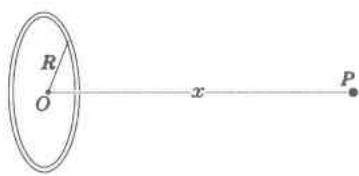
\includegraphics[width=0.3\linewidth]{figures/习题1-25.jpg}
\end{center}


\vfill

\textbf{1-26.} 半径为 $R$ 的圆面均匀带电，电荷的面密度为 $\sigma_{\mathrm{e}}$

(1) 求轴线上离圆心的坐标为 $x$ 处的场强；

(2) 在保持 $\sigma_{e}$ 不变的情况下, 当 $R \to 0$ 和 $R \to \infty$ 时结果各如何?

(3) 在保持总电荷 $Q=\pi R^{2}\sigma_{e}$ 不变的情况下，当 $R\to0$ 和 $R\to\infty$ 时结果各如何？

(4) 求轴线上电势 $U(x)$ 的分布，并画出 $U-x$ 曲线。

\vfill
\newpage

\textbf{1-30.} 在氢原子中, 正常状态下电子到质子的距离为 $5.29 \times 10^{-11} \mathrm{~m}$ , 已知氢原子核 (质子) 和电子带电荷量各为 $\pm e (e = 1.60 \times 10^{-19} \mathrm{C})$ 。把氢原子中的电子从正常状态下拉开到无穷远处所需的能量, 叫做氢原子的电离能。求此电离能是多少 $\mathrm{eV}$ ?

\vfill

\textbf{1-32.} 在绝对温度为 $T$ 时，微观粒子热运动能量具有 $kT$ 的数量级（玻耳兹曼常量 $k = 1.38 \times 10^{-23} \mathrm{~J} / \mathrm{K}$ ）。有时人们把能量 $kT$ 折合成 $\mathrm{eV}$ ，就说温度 $T$ 为若干 $\mathrm{eV}$ . 问：

(1) $T=1\mathrm{eV}$ 相当于多少K?

(2) $T=50\ keV$ 相当于多少K?

(3) 室温 $(T \approx 300\mathrm{K})$ 相当于多少 $\mathrm{eV}$?

\vfill
\newpage

\textbf{1-34.} 电视显像管的第二和第三阳极是两个直径相同的同轴金属圆筒。两电极间的电场即为显像管中的主聚焦电场。本题图中所示为主聚焦电场中的等势面，数字表示电势值。试用直尺量出管轴上各等势面间的距离，并求出相应的电场强度。
\begin{center}
    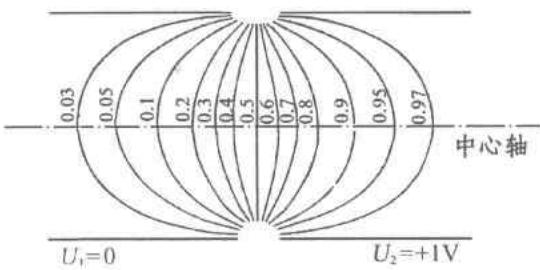
\includegraphics[width=0.3\linewidth]{figures/习题1-34.jpg}
\end{center}


\vfill

\textbf{1-36.} 如本题图所示，在半径为 $R_{1}$ 和 $R_{2}$ 的两个同心球面上，分别均匀地分布着电荷 $Q_{1}$ 和 $Q_{2}$ ，

(1) 求 I、II、III 三个区域内的场强分布。

(2) 若 $Q_{1} = -Q_{2}$ ，情况如何？画出此情形的下 $E-r$ 曲线。

(3) 按情形(2) 求 I、II、III 三个区域内的电势分布, 并画出 $U-r$ 曲线。

\begin{center}
    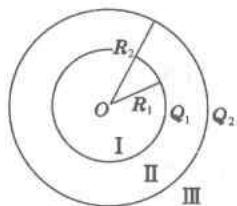
\includegraphics[width=0.2\linewidth]{figures/习题1-36.jpg}
\end{center}

\vfill
\newpage

\textbf{1-37.} 一对无限长的共轴直圆筒，半径分别为 $R_{1}$ 和 $R_{2}$ ，筒面上都均匀带电。沿轴线单位长度的电荷量分别为 $\lambda_{1}$ 和 $\lambda_{2}$ .

(1) 求各区域内的场强分布。

(2) 若 $\lambda_{1} = -\lambda_{2}$ ，情况如何？画出此情形的 $E-r$ 曲线。

(3) 按情形(2) 求两筒间的电势差和电势分布。

\vfill

\textbf{1-39.} 设气体放电形成的等离子体圆柱内的体电荷分布可用下式表示：
$$
\rho_ {\mathrm{e}} (r) = \frac {\rho_ {0}}{\left[ 1 + \left(\frac {r}{a}\right) ^ {2} \right] ^ {2}},
$$
式中 $r$ 是到轴线的距离， $\rho_{0}$ 是轴线上的 $\rho_{e}$ 值，a 是个常量（它是 $\rho_{e}$ 减少到 $\rho_{0}/4$ 处的半径）。

(1) 求场强分布。

(2) 以轴线为电势零点求电势分布。

\vfill
\newpage

\textbf{1-40.} 一电子二极管由半径 $r = 0.50\mathrm{mm}$ 的圆柱形阴极K和套在阴极外同轴圆筒形的阳极A构成，阳极的半径 $R = 0.45\mathrm{cm}$ . 阳极电势比阴极高 $300\mathrm{V}$ . 设电子从阴极发射出来时速度很小，可忽略不计。求：

(1) 电子从 $\mathrm{K}$ 向 A 走过 2.0 $\mathrm{mm}$ 时的速度。

(2) 电子到达 $\mathrm{A}$ 时的速度。

\vfill

\textbf{1-41.} 如本题图所示，一对均匀、等量异号的平行带电平面。若其间距离 $d$ 远小于带电平面的线度时，这对带电面可看成是无限大的。这样的模型可叫做电偶极层。求场强和电势沿垂直两平面的方向 $x$ 的分布，并画出 $E - x$ 和 $U - x$ 曲线（取离两平面等距的 $O$ 点为参考点，令该处电势为零）。

\begin{center}
    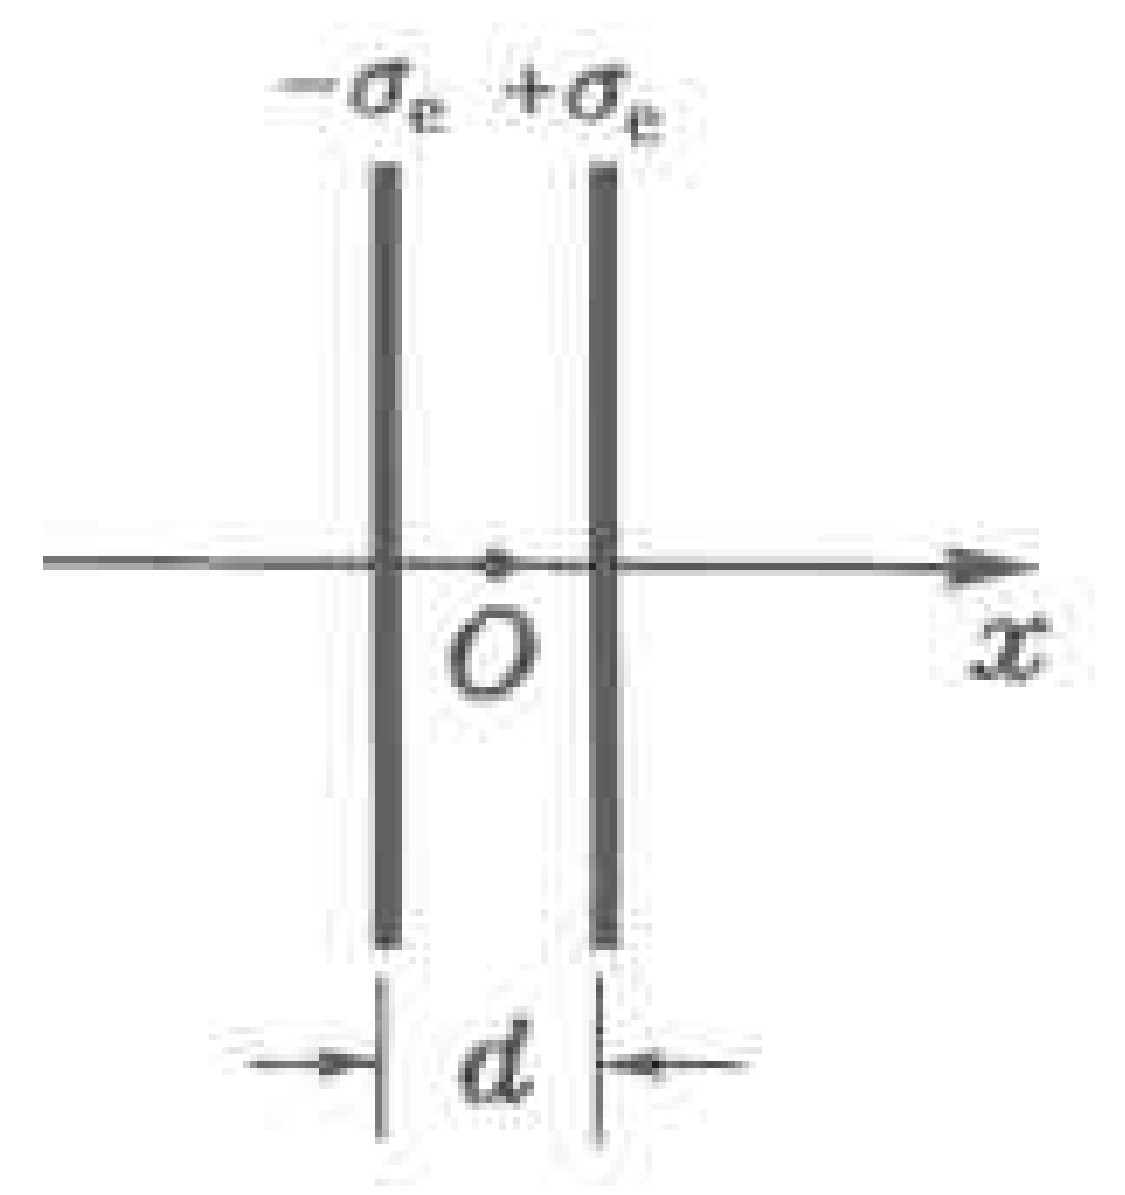
\includegraphics[width=0.2\linewidth]{figures/习题1-41.jpg}
\end{center}


\vfill
\newpage

\textbf{1-42.} 在半导体PN结附近总是堆积着正、负电荷，在N区内有正电荷，P区内有负电荷，两区电荷的代数和为零。我们把PN结看成是一对带正、负电荷的无限大平板，它们相互接触（见本题图）。取坐标 $x$ 的原点在P、N区的交界面上，N区的范围是 $-x_{\mathrm{N}} \leqslant x \leqslant 0$ ，P区的范围是 $0 \leqslant x \leqslant x_{\mathrm{p}}$ 。设两区内电荷体分布都是均匀的：
$$
\left\{ \begin{array}{l l} {N \text {区}:} & {\rho_ {\mathrm{e}} (x) = n _ {\mathrm{N}} e,} \\ {P \text {区}:} & {\rho_ {\mathrm{e}} (x) = - n _ {\mathrm{p}} e.} \end{array} \right.
$$
(突变结模型)
这里 $n_{N}$ 、 $n_{P}$ 是常量，且 $n_{N}x_{N}=n_{P}x_{P}$ （两区电荷数量相等）。试证明：

(1) 电场的分布为
$$
\left\{ \begin{array}{l l} {N \text {区}:} & {E (x) = \frac {n _ {\mathrm{N}} e}{\varepsilon_ {0}} (x _ {\mathrm{N}} + x),} \\ {P \text {区}:} & {E (x) = \frac {n _ {\mathrm{P}} e}{\varepsilon_ {0}} (x _ {\mathrm{P}} - x).} \end{array} \right.
$$
并画出 $\rho_{\mathrm{e}}(x)$ 和 $E(x)$ 随 $x$ 变化的曲线来。

(2)PN结内的电势分布为

$$
\left\{ \begin{array}{l l} N \text {区}: & U (x) = - \frac {n _ {\mathrm{N}} e}{\varepsilon_ {0}} \Big (x _ {\mathrm{N}} x + \frac {1}{2} x ^ {2} \Big), \\ P \text {区}: & U (x) = - \frac {n _ {\mathrm{P}} e}{\varepsilon_ {0}} \Big (x _ {\mathrm{P}} x - \frac {1}{2} x ^ {2} \Big). \end{array} \right.
$$
这公式是以何处为电势零点的？PN结两侧的电势差多少？
\begin{center}
    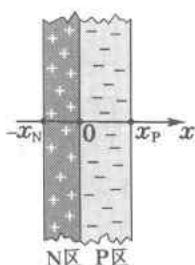
\includegraphics[width=0.2\linewidth]{figures/习题1-42b.jpg}
\end{center}

\vfill
\newpage

\textbf{1-43.} 如果在上题中电荷的体分布为
$$
\left\{ \begin{array}{l l} {\mathrm{PN}   \text {外}:} & {\rho (  x  ) = 0  ,} \\ {- x _ {\mathrm{N}} \leqslant x \leqslant x _ {\mathrm{P}}:} & {\rho (  x  ) = - e a x.} \end{array} \right.
$$
(线性缓变结模型)
这里 a 是常量， $x_{N}=x_{P}$ （为什么？），统一用 $x_{m}/2$ 表示。试证明：
(1) 电场的分布为
$$
E (x) = \frac {a e}{8 \varepsilon_ {0}} (x _ {\mathrm{m}} ^ {2} - 4 x ^ {2}),
$$
并画出 $\rho_{\mathrm{e}}(x)$ 和 $E(x)$ 随 $x$ 变化的曲线来。
(2)PN结内的电势分布为
$$
U (x) = \frac {a e}{2 \varepsilon_ {0}} \left(\frac {x ^ {3}}{3} - \frac {x _ {\mathrm{m}} ^ {2} x}{4}\right),
$$
这公式是以何处为电势零点的？PN结两侧的电势差多少？

\vfill


\textbf{1-44.} 证明: 在真空静电场中凡是电场线都是平行直线的地方, 电场强度的大小必定处处相等; 或者换句话说, 凡是电场强度的方向处处相同的地方, 电场强度的大小必定处处相等。
【提示:利用高斯定理和作功与路径无关的性质,分别证明沿同一电场线和沿同一等势面上两点的场强相等。】

\vfill\newpage

\textbf{1-45.} 如本题图所示,一平行板电容器充电后,A、B两极板上电荷的面密度分别为 $\sigma_{e}$ 和 $-\sigma_{e}$ . 设 P 为两板间任一点,略去边缘效应(即可把两板当作无限大),

(1) 求 A 板上的电荷在 P 点产生的电场强度 $E_{A}$ ;

(2) 求 B 板上的电荷在 P 点产生的电场强度 $E_{B}$ ;

(3) 求 A、B 两板上的电荷在 P 点产生的电场强度 E；

(4) 若把 B 板拿走，A 板上电荷如何分布？A 板上的电荷在 P 点产生的电场强度为多少？

\begin{center}
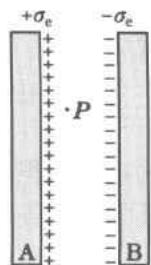
\includegraphics[width=0.15\linewidth]{figures/习题1-45a.jpg}
\end{center}
\vfill


\textbf{1-46}. 对于两个无限大的平行平面带电导体板来说，

(1) 证明：相向的两面（本题图中2和3）上，电荷的面密度总是大小相等而符号相反；

(2) 证明：相背的两面（本题图中1和4）上，电荷的面密度总是大小相等而符号相同；

(3) 若左导体板带电 $+3\mu C/m^{2}$ ，右导体板带电 $+7\mu C/m^{2}$ ，求四个表面上的电荷。

\begin{center}
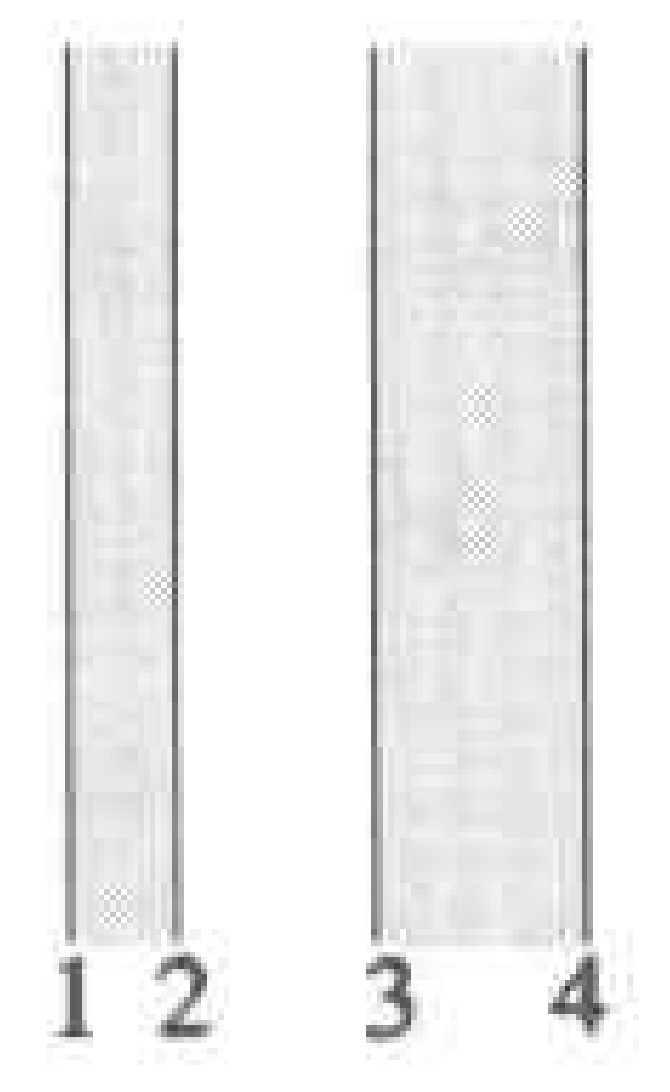
\includegraphics[width=0.15\linewidth]{figures/习题1-46.jpg}
\end{center}

\vfill\newpage

\textbf{1-47.} 两平行金属板分别带有等量的正负电荷。两板的电势差为 $120\mathrm{V}$ ，两板的面积都是 $3.6\mathrm{cm}^2$ ，两板相距 $1.6\mathrm{mm}$ 。略去边缘效应，求两板间的电场强度和各板上所带电荷量。

\vfill

\textbf{1-48.} 两块带有等量异号电荷的金属板a和b，相距 $5.0\mathrm{mm}$ ，两板的
面积都是 $150cm^{2}$ ，电荷量的数值都是 $2.66\times10^{-8}C$ ，a板带正电并接地（见本题图）。以地的电势为零，并略去边缘效应，问：

(1) $b$ 板的电势是多少?

(2) $a$、$b$间离 $a$ 板 $1.0\mathrm{mm}$ 处的电势是多少?

\begin{center}
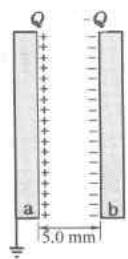
\includegraphics[width=0.15\linewidth]{figures/习题1-48.jpg}
\end{center}

\vfill
\newpage

\textbf{1-49.} 三平行金属板 A、B 和 C, 面积都是 $200 \mathrm{~cm}^{2}$ , AB 相距 $4.0 \mathrm{~mm}$ , AC 相距 $2.0 \mathrm{~mm}$ , BC 两板都接地 (见本题图)。如果使 A 板带正电 $3.0 \times 10^{-7} \mathrm{C}$ , 在略去边缘效应时, 问 B 板和 C 板上感应电荷各是多少? 以地的电势为零, 问 A 板的电势是多少?

\vfill

\textbf{1-50.} 点电荷 $q$ 处在导体球壳的中心，壳的内外半径分别为 $R_{1}$ 和 $R_{2}$ （见本题图）。求场强和电势的分布，并画出 $E - r$ 和 $U - r$ 曲线。
\begin{center}
    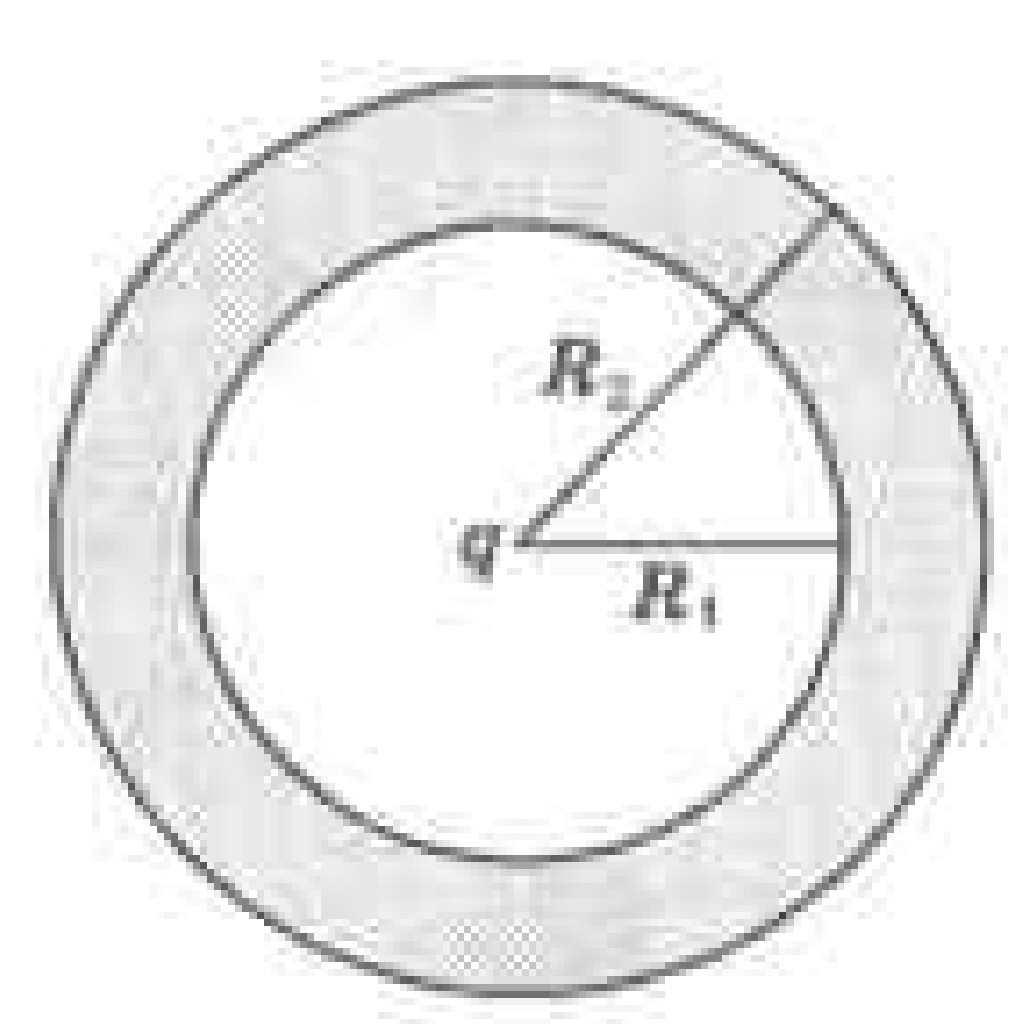
\includegraphics[width=0.2\linewidth]{figures/习题1-50.jpg}
\end{center}

\vfill
\newpage



\textbf{1-51.} 在上题中, 若 $q = 4.0 \times 10^{-10} \mathrm{C}$ , $R_{1} = 2.0 \mathrm{cm}$ , $R_{2} = 3.0 \mathrm{cm}$ ,

(1) 求导体球壳的电势；

(2) 求离球心 $r = 1.0 cm$ 处的电势；

(3) 把点电荷移开球心 1.0cm, 求导体球壳的电势。

\vfill


\textbf{1-52.} 半径为 $R_{1}$ 的导体球带有电荷 $q$ ，球外有一个内外半径为 $R_{2}, R_{3}$ 的同心导体球壳，壳上带有电荷 $Q$ （见本题图）。

(1) 求两球的电势 $U_{1}$ 和 $U_{2}$ ;

(2) 求两球的电势差 $\Delta U$ ;

(3)以导线把球和壳连接在一起后， $U_{1}$ 、 $U_{2}$ 和 $\Delta U$ 习题 1-52 分别是多少？

(4) 在情形(1)、(2)中, 若外球接地, $U_{1}, U_{2}$ 和 $\Delta U$ 为多少?

(5) 设外球离地面很远, 若内球接地, 情况如何?

\begin{center}
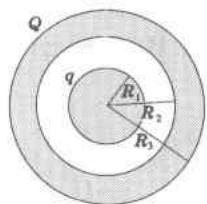
\includegraphics[width=0.25\linewidth]{figures/习题1-52a.jpg}
\end{center}

\vfill\newpage


\textbf{1-53.} 在上题中设 $q = 1.0 \times 10^{-10} \mathrm{C}$ , $Q = 11 \times 10^{-10} \mathrm{C}$ , $R_{1} = 1.0 \mathrm{~cm}$ , $R_{2} = 3.0 \mathrm{~cm}$ , $R_{3} = 4.0 \mathrm{~cm}$ , 试计算各情形中的 $U_{1}, U_{2}$ 和 $\Delta U$ , 并画出 $U - r$ 曲线来。

\vfill


\textbf{1-54.} 假设范德格拉夫起电机的球壳与传送带上喷射电荷的尖针之间的电势差为 $3.0 \times 10^{6} \mathrm{~V}$ , 如果传送带迁移电荷到球壳上的速率为 $3.0 \times 10^{-3} \mathrm{C} / \mathrm{s}$ , 则在仅考虑电力的情况下, 必须用多大的功率来开动传送带?


\vfill\newpage

\textbf{1-55.} 范德格拉夫起电机的球壳直径为 $1.0\mathrm{m}$ , 空气的击穿场强为 $30\mathrm{kV/cm}$ (即球表面的场强超过此值, 电荷就会从空气中漏掉)。这起电机最多能达到多高的电势?

\vfill


\textbf{1-57.} 如本题图所示, 平行板电容器两极板的面积都是 $S$ , 相距为 $d$ , 其间有一厚为 $t$ 的金属片。略去边缘效应。

(1) 求电容 C;

(2) 金属片离极板的远近有无影响?
\begin{center}
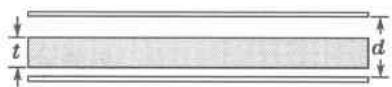
\includegraphics[width=0.3\linewidth]{figures/习题1-57.jpg}
\end{center}
\vfill\newpage

\textbf{1-58.} 如本题图所示,一电容器两极板都是边长为 $a$ 的正方形金属平板,两板不严格平行,其间有一夹角 $\theta$ . 证明: 当 $\theta \ll d / a$ 时,略去边缘效应,它的电容为

$$
C = \varepsilon_ {0} \frac {a ^ {2}}{d} \left(1 - \frac {a \theta}{2 d}\right).
$$
\begin{center}
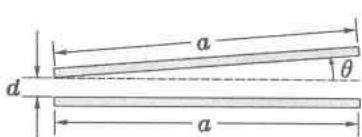
\includegraphics[width=0.3\linewidth]{figures/习题1-58.jpg}
\end{center}

\vfill


\textbf{1-59.} 半径都是 $a$ 的两根平行长直导线相距为 $d(d \gg a)$ ，求单位长度的电容。

\vfill\newpage

\textbf{1-60.} 证明：同轴圆柱形电容器两极的半径相差很小（即 $R_{\mathrm{B}} - R_{\mathrm{A}} \ll R_{\mathrm{A}}$ ）时，它的电容公式$C = \dfrac{2\pi\varepsilon_0 L}{\ln{R_b/R_A}}$趋于平行板电容公式$C = \dfrac{\varepsilon_0 S}{d}$。

\vfill


\textbf{1-61.} 证明: 同心球形电容器两极的半径相差很小(即 $R_{\mathrm{B}} - R_{\mathrm{A}} \ll R_{\mathrm{A}}$ )时, 它的电容公式$C = \dfrac{4\pi\varepsilon_0 R_A R_B}{R_B - R_A}$ 趋于平行板电容公式$C = \dfrac{\varepsilon_0 S}{d}$。

\vfill\newpage

\textbf{1-62.} 一球形电容器内外两壳的半径分别为 $R_{1}$ 和 $R_{4}$ ，今在两壳之间放一个内外半径分别为 $R_{2}$ 和 $R_{3}$ 的同心导体球壳（见本题图）。

(1)给内壳 $(R_{1})$ 以电量Q，求 $R_{1}$ 和 $R_{4}$ 两壳的电势差；

(2) 求以 $R_{1}$ 和 $R_{4}$ 为两极的电容。

\begin{center}
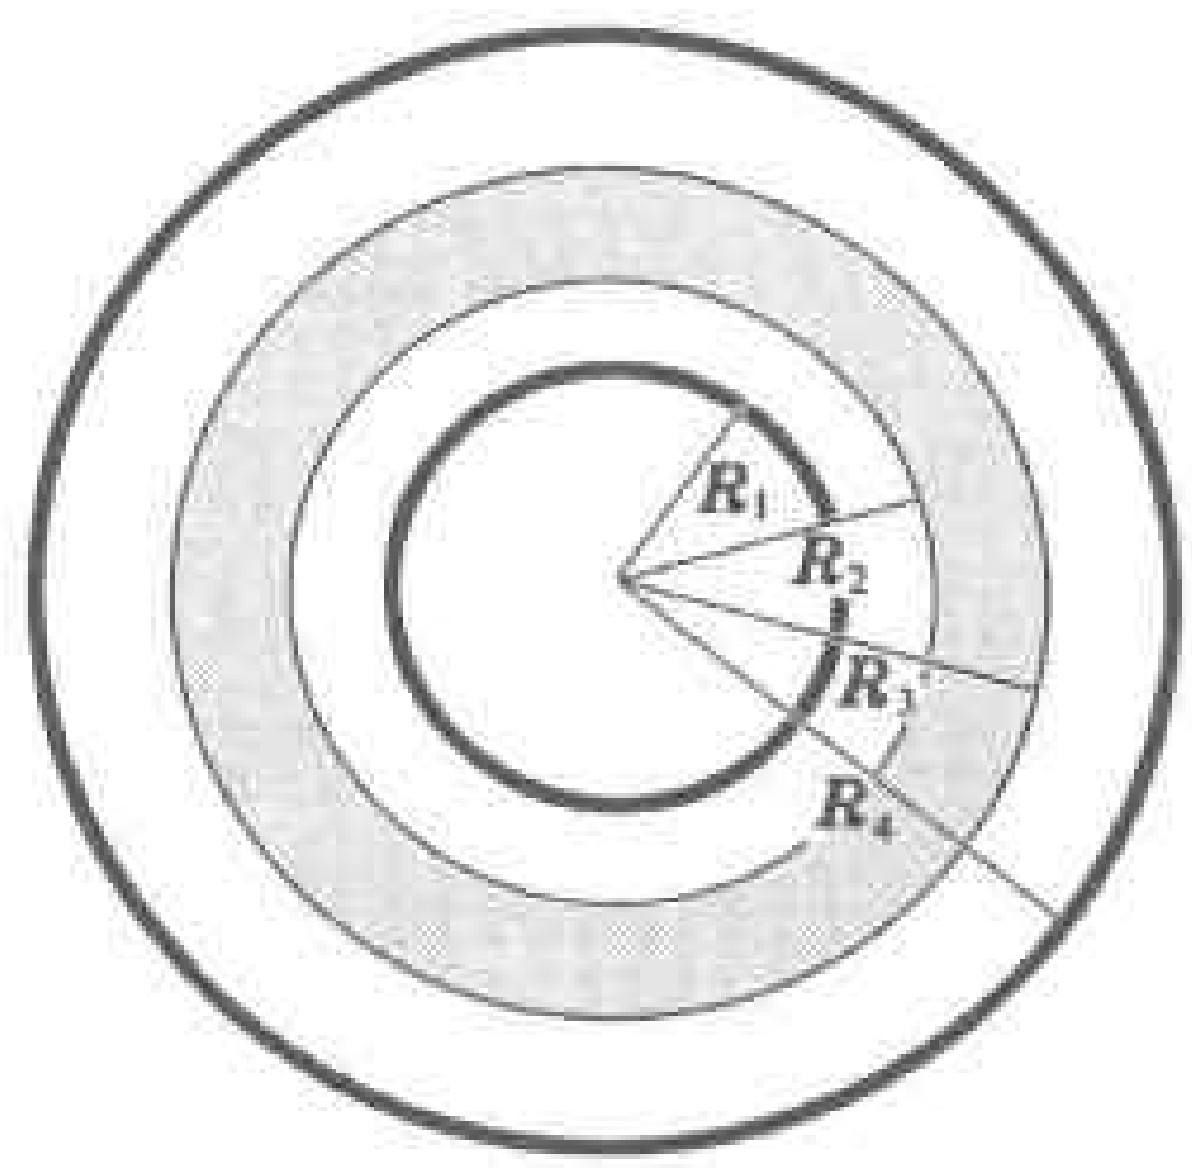
\includegraphics[width=0.2\linewidth]{figures/习题1-62.jpg}
\end{center}

\vfill


\textbf{1-63.} 半径为 $2.0\mathrm{cm}$ 的导体球外套有一个与它同心的导体球壳，壳的内外半径分别为 $4.0\mathrm{cm}$ 和 $5.0\mathrm{cm}$ ，球与壳间是空气。壳外也是空气，当内球的电量为 $3.0\times 10^{-8}\mathrm{C}$ 时，

(1) 这个系统储藏了多少电能？

(2) 如果用导线把壳与球联在一起, 结果如何?

\vfill\newpage

\textbf{1-64.} 激光闪光灯的电源线路如本题图所示，由电容器 $C$ 储存的能量，通过闪光灯线路放电，给闪光提供能量。电容 $C = 6000\mu \mathrm{F}$ ，火花间隙击穿电压为 $2000\mathrm{V}$ ，问 $C$ 在一次放电过程中，能放出多少能量？
\begin{center}
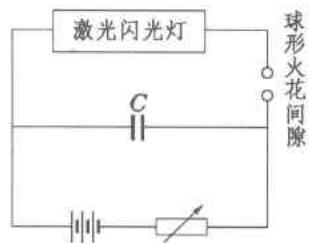
\includegraphics[width=0.3\linewidth]{figures/习题1-64.jpg}
\end{center}


\vfill


\textbf{1-65.} 地面可看成是无穷大的导体平面，一均匀带电无限长直导线平行地面放置（垂直于本题图），求空间的电场强度、电势分布和地表面上的电荷分布。
\begin{center}
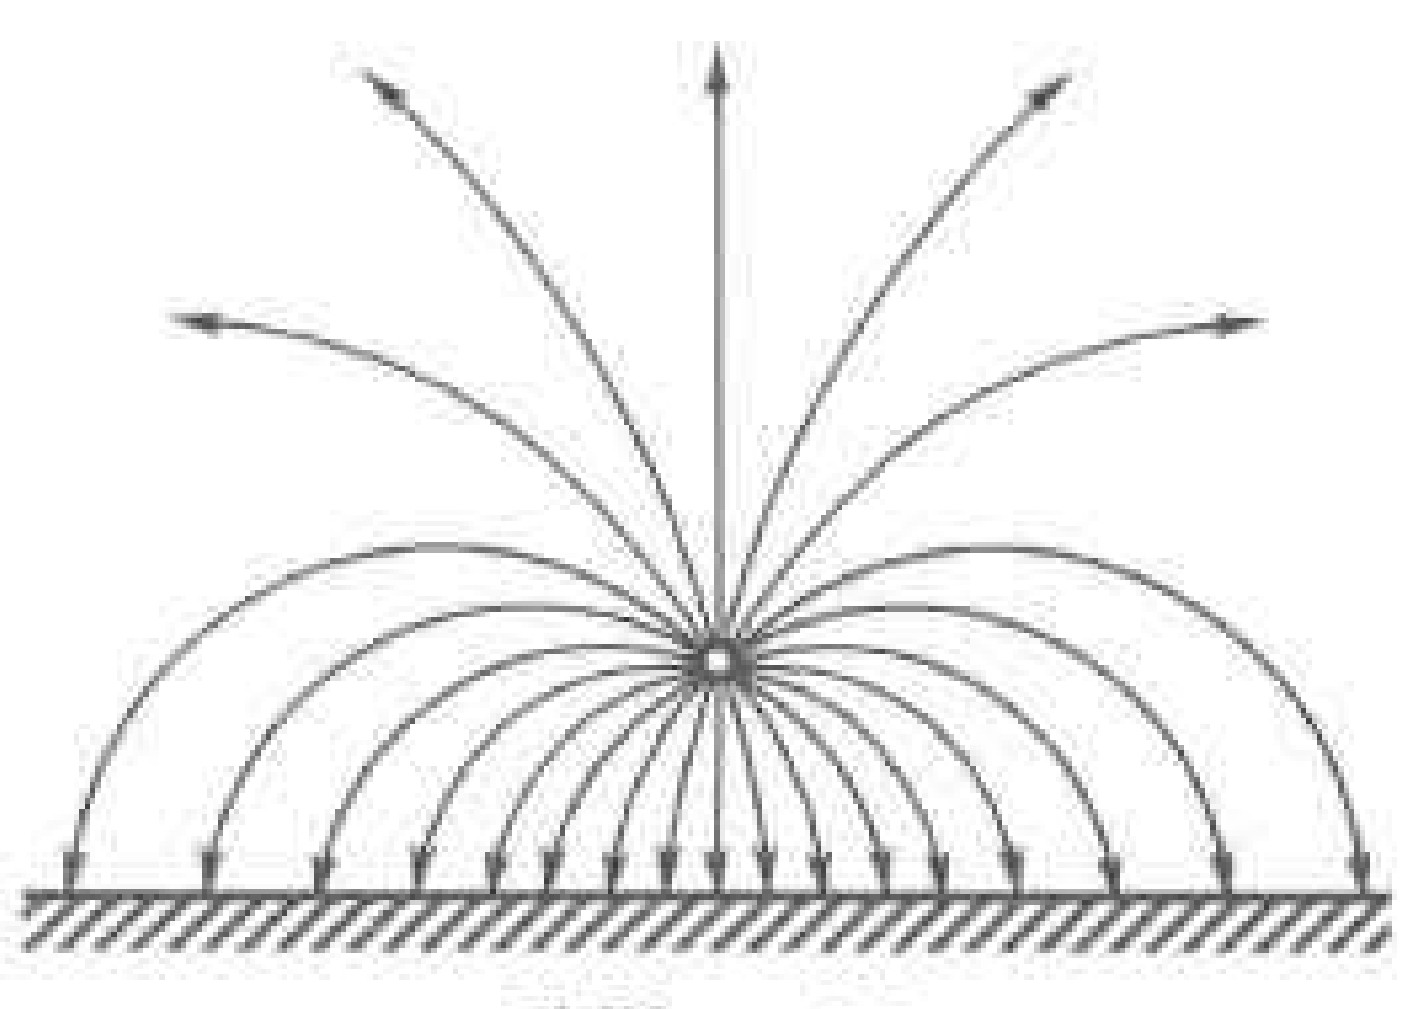
\includegraphics[width=0.2\linewidth]{figures/习题1-65.jpg}
\end{center}

\vfill\newpage

\textbf{1-66.} 本题图中两边为电导率很大的导体，中间两层是电导率分别为 $\sigma_{1}$ 、 $\sigma_{2}$ 的均匀导电介质，其厚度分别为 $d_{1}$ 、 $d_{2}$ ，导体的截面积为 $S$ ，通过导体的恒定电流为 $I$ ，求：

(1) 两层导电介质中的场强 $E_{1}$ 和 $E_{2}$ ;

(2) 电势差 $U_{AB}$ 和 $U_{BC}$ .
\begin{center}
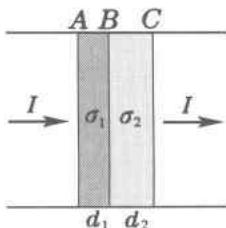
\includegraphics[width=0.2\linewidth]{figures/习题1-66.jpg}
\end{center}
\vfill


\textbf{1-67.} 同轴电缆内、外半径分别为 $a$ 和 $b$ , 其间电介质有漏电阻, 电导率为 $\sigma$ , 如本题图所示。求长度为 $l$ 的一段电缆内的漏阻。
\begin{center}
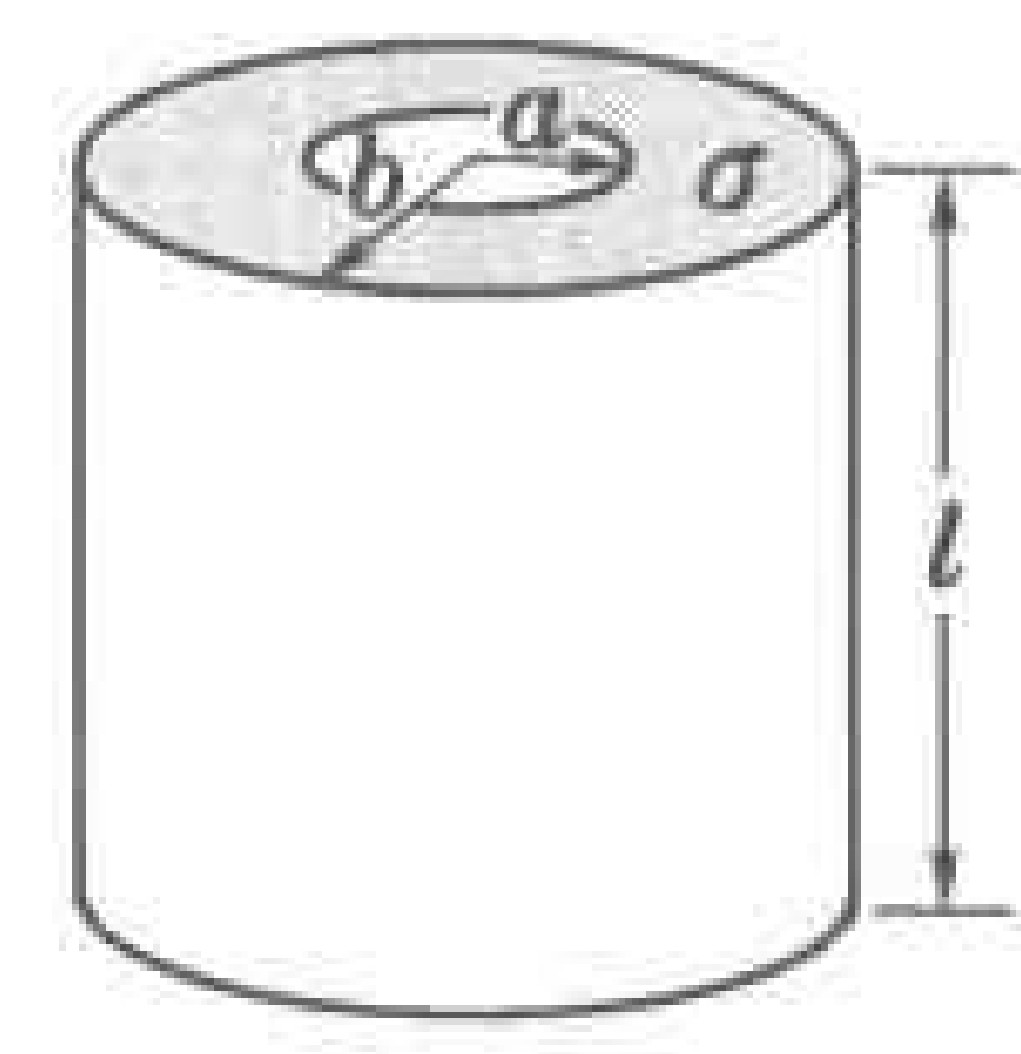
\includegraphics[width=0.2\linewidth]{figures/习题1-67.jpg}
\end{center}

\vfill\newpage